\documentclass[a4paper,10pt,twoside,fleqn]{article}

% Note that if you want to use the \begin{equation} ... \end{equation}
% environment, you will have to include fleqn in the
% \documentclass[...]{...} options! 
% The top of your LaTeX file should then look like this:
% \documentclass[a4paper,10pt,twoside,fleqn]{article}
\usepackage[utf8]{inputenc}
\usepackage{clin}        % Stylefile for CLIN Journal
\usepackage{harvard}     % Bibliography Stylefile
%\usepackage{...,cgloss4e,avm,trees,tree-dvips,gb4e,ipa,graphicx}
                         % Whatever other packages you need
% Harvard:
% \cite{Covington}             (Covington 1994)
% \citeasnoun{Covington}       Covington (1994)
% \citeyear{Covington}         (1994)

\pagestyle{empty}

%%% own packages
\usepackage{booktabs}
\usepackage{chngcntr}
\usepackage{rotating}
\usepackage[section]{placeins}
\usepackage[super]{nth}
\usepackage{wrapfig}

%%% commands
\newcommand{\overbar}[1]{\mkern 2.0mu\overline{\mkern-2.0mu#1\mkern-2.0mu}\mkern 2.0mu}


\begin{document}

\title{Towards Distinctive and Typical Style Features in Authorship}


\author{Carmen Klaussner$^*$ \email{klaussnc@tcd.ie}\\
{\normalsize \bf \c{C}a\u{g}ri \c{C}öltekin}$^{**}$ \email{c.coltekin@rug.nl}\\
{\normalsize \bf John Nerbonne}$^{**}$ \email{j.nerbonne@rug.nl}
\AND \addr{$^*$Trinity College Dublin, Ireland}
\AND \addr{$^{**}$University of Groningen, The Netherlands} }


\maketitle\thispagestyle{empty} % extra pagestyle command for first page

%To be filled in by the editors
%Please leave commented out
%\jmlrheading{vol}{year}{pages}{Submission date}{Publication date}{authors}
%\copyright

\begin{abstract}
Detection of stylistic elements in authorship studies is hampered
by the lack of a gold standard that would otherwise enable us to 
clearly evaluate our findings. In absence thereof, one generally 
resorts to choosing items for which an author shows a 
characteristic usage compared with other writers. 
In this line of work, we present both a measure for determining 
characteristic elements of an author that he uses consistently
over different works by examining different types of features, 
both lexical and syntactic ones.
For evaluation, we test the separation ability of the selected 
features by clustering the data set on their basis.

We apply both feature selection and evaluation in two different
studies of authorship. In the first, we compare Charles Dickens 
and Wilkie Collins, while the second one is contrasting the 
styles of Henry James and Mark Twain. Testing separation ability 
in clustering on highly representative and distinctive features 
returns results very close to the ideal clustering result.
\end{abstract}




\section{Introduction}
% this needs to include more references
The concept of \emph{style} in studies of authorship refers to the 
something like the feel of a piece of text, which might be less
tangible than style in other disciplines, such as art or music, 
where we use \emph{language} to express aspects of a 
painting or a piece of music, whereas for style in writing, 
we have to use the same tools that were used to create it. 

While traditional studies of authorship involve individual persona
judging upon what constitutes the style of an author, non-traditional
studies employ statistical techniques to discover the style of
an author. 
In either scenario, the development and investigation of suitable
methods of detection is hampered by the lack of a gold standard,
that would be able to indicate the method's closeness to 
returning true stylistic elements of an author. 
In absence thereof, the weight lies primarily on the method's 
theoretical appropriateness in the way it selects stylistic 
markers, which results in the need to understand our methods 
as well as their implications. 

\emph{Consistency} of stylistic markers has been somewhat of 
a central theme to studies of authorship, such as in early 
studies \cite{Mosteller2008}, which also emphasised collecting
larger number of markers to increase reliability of the result.
This has been continues in more recent studies as in 
the development of Burrow's Delta \cite{Burrows2002delta} 
and Zeta \cite{Burrows2007all} measures that build on
features representative for an author over a given number
of his texts, while distinguishing him from another/other 
author(s).

In this work, we consider \emph{Representativeness \& Distinctiveness}
\cite{prokic2012detecting}, a technique originating in dialectometry 
to select an author’s consistent features that are at the same time
also distinctive with respect to an opposing author’s sample.
Further, we propose a heuristic method for evaluation of those
selected features intended to measure how well they are able to
separate the data set into the correct groupings. 
As part of the analysis, we include both lexical and syntactic ones, 
such as simple word uni-grams, but also Part-of-Speech (POS) 
bi-grams/tri-grams.
The data consists of two separate authorship sets, where the first
consists of texts by two British authors, Charles Dickens and
Wilkie Collins and the second comprises writings by the two
American authors, Henry James and Mark Twain. 
%references of studies on those authors

Thus, in section~\ref{sec:data}, we describe the two data sets, while we 
introduce \emph{Representativeness \& Distinctiveness} 
in section~\ref{sec:method}. Further, section~\ref{sec:evaluation}
introduces and illustrates our proposed method of evaluation. 
Finally, in section~\ref{sec:experiments}, we describe our experiments
and results with respect to the two data sets and section~\ref{sec:conclusion}
closes the discussion. 


\section{The Data Sets} \label{sec:data}
For this study, we built two different author sets, one comparing Charles Dickens
and contemporary writer Wilkie Collins and the other one opposing Henry James 
to fellow American writer Mark Twain. 
All data was obtained from \emph{Project Gutenberg}\footnote{http://www.gutenberg.org/}
and the \emph{Internet Archive}\footnote{https://archive.org/}.

\subsection{Dickens vs. Collins}
% connection Dickens/Collins
Table~\ref{table:Dickens-data} and table~\ref{table:Collins-data} show Dickens'
and Collins' data set respectively, both comprising 27 documents.
Dickens' data set does not only contain documents by himself, but three books, namely, 
\emph{A Budget of Christmas Tales}, \emph{A House to Let} and \emph{No Thoroughfare}
are collaborations, where Dickens seems to have been main author.
In particular, the last two also include Wilkie Collins as author, where 
\emph{No Thoroughfare} was written by only Dickens and Collins. 
These were included, since they might be interesting with respect to stylistic properties.
If both authors persist in terms of style, these should be somewhat more difficult 
to classify than those written by only one of them.  
% exclude these from selection set 




% Dickens vs. Collins
\begin{table}[!ht]
%\caption{Dickens' data set.}
      \label{table:Dickens-data}
      \small
\begin{tabular}{c l l l} \\\hline \hline
\textbf{No.} 	& \textbf{Author} 	& \textbf{Texts} 			& \textbf{Abbr.} \\ \hline
1   		& Dickens 		& Bleak House 				& D1023     \\
2   		& Dickens		& Great Expectations			& D1400      \\
3		& Dickens      		& Little Dorrit     			& D963       \\
4		& Dickens      		& David Copperfield     		& D766        \\
5		& Dickens      		& A Christmas Carol     		& D19337       \\
6   		& Dickens		& Life And Adventures Of Martin Chuzzlewit	& D968        \\
7		& Dickens		& The Mystery of Edwin Drood		& D564   \\
8		& Dickens      		& A Tale of Two Cities                  & D98      \\
9		& Dickens		& Master Humphrey's Clock		& D588           \\
10		& Dickens		& The Battle of Life: A Love Story      & D40723              \\
11		& Dickens		& Life And Adventures Of Nicholas Nickleby	& D967          \\  
12		& Dickens		& Barnaby Rudge      			& D917             \\
13		& Dickens		& Sketches of Young Couples		& D916        \\
14		& Dickens		& The Uncommercial Traveller            & D914           \\
15		& Dickens		& Our Mutual Friend			& D883           \\
16		& Dickens		& Pictures From Italy			& D650    \\
17		& Dickens		& Sketches by Boz			& D882      \\
18		& Dickens		& A Child's History of England       	& D699  \\
19		& Dickens		& Reprinted Pieces			& D872   \\
20		& Dickens		& Dombey and Son			& D821     \\
21		& Dickens		& Oliver Twist				& D730        \\
22		& Dickens		&The Old Curiosity Shop			& D700         \\
23		& Dickens		& American Notes			& D675         \\
24		& Dickens		&The Pickwick Papers			& D580           \\
25		& Dickens    (et al.)   & A Budget of Christmas Tales		& Dal28198         \\
26		& Dickens (et al.)	& A House to Let			& Dal2324     \\
27		& Dickens (/Collins)     & No Thoroughfare			& DC1423       \\ \bottomrule
\end{tabular}
\end{table}


\begin{table}[!ht]
\caption{Collins' data set.}
\label{table:Collins-data}
\small
\begin{tabular}{c l l l } \\\hline \hline
\textbf{No.}	& \textbf{Author} 		& \textbf{Texts} 		& \textbf{Abbr.} \\ \hline
1		& Collins       		& After Dark			& C1626    \\
2		& Collins			& Antonina			& C3606        \\
3		& Collins			& Armadale			& C1895  \\
4		& Collins			& Man and Wife			& C1586      \\
5		& Collins			& Little Novels			& C1630    \\
6		& Collins			& Jezebel's Daughter		& C3633    \\
7		& Collins			& I Say No			& C1629       \\
8		& Collins			& Hide and Seek			& C7893  \\
9		& Collins			& Basil				& C4605 \\
10		& Collins			& A Rogue's Life		& C1588     \\
11		& Collins			& The Woman in White		& C583         \\
12		& Collins			& The Two Destinies		& C1624    \\
13		& Collins			& The Queen of Hearts		& C1917        \\
14		& Collins			& The New Magdalen		& C1623     \\
15		& Collins			& The Moonstone			& C155         \\
16		& Collins			& The Legacy of Cain		& C1975       \\
17		& Collins			& The Law and the Lady		& C1622         \\
18		& Collins			& The Haunted Hotel: A Mystery of Modern Venice	&    C170              \\
19		& Collins			& The Fallen Leaves		& C7894           \\
20		& Collins			& The Evil Genius		& C1627           \\
21		& Collins			& No Name			& C1438        \\
22		& Collins			& Poor Miss Finch		& C3632           \\
23		& Collins			& Rambles Beyond Railways	& C28367         \\
24		& Collins			& The Black Robe		& C1587      \\
25		& Collins			& Miss or Mrs.?			& C1621          \\
26		& Collins			& My Lady's Money		& C1628         \\
27		& Collins			& The Dead Alive		& C7891        \\
\bottomrule
\end{tabular}  
\end{table}


\subsection{James vs. Twain}
While Dickens and Collins seemed to have been close enough to collaborate on work,
this is a highly unlikely scenario for Henry James and Mark Twain. 
Although both being American writers close in age, they did not seemed to have
approved of each other as artists \cite{canby1951turn}. 
It is interesting to investigate to what extent this mutual dislike and 
disapprobation of each other 's work manifests itself in their writings
and what elements separate them. 
Table~\ref{table:Twain-data} and table~\ref{table:Twain-data} show 
James' and Twain's data sets, where James is represented with 25 and Twain
with 21 works. 


%James vs. Twain
\begin{table}[!htb]
    %\caption{Twain' and James' data set as part of the Twain vs. James' comparison.}
   % \label{table:TJ}
    \begin{minipage}{.62\linewidth}
    \centering
      \caption{Twain's data set.} %necessary???
      
      \label{table:Twain-data}
\begin{tabular}{c l l l} \\\hline \hline
\textbf{No.} 	& \textbf{Author} 	& \textbf{Texts} 			& \textbf{Abbr.} \\ \hline
1		&Twain			&Innocents Abroad			& T-ia\\ 
2		&Twain			&The Gilded Age: A Tale of Today	& T-tgaatot\\ 
3		&Twain			&Sketches New and Old			& T-snao\\
4		&Twain			&The Adventures of Tom Sawyer		& T-taots\\ 
5		&Twain			&A Tramp Abroad				& T-ata\\ 
6		&Twain			&Roughing It				& T-ri \\ 
7		&Twain			&The Prince and the Pauper		& T-tpatp\\ 
8		&Twain			&Life on the Mississippi		& T-lotm\\ 
9		&Twain			&The Adventures of Huckleberry Finn	& T-taohf\\ 
10		&Twain			&A Connecticut Yankee in King Arthur's Court& T-acyikac\\  
11		&Twain			&The American Claimant			& T-tac\\  
12		&Twain			&The Tragedy of Pudd'nhead Wilson	&T-ttopw\\   
13		&Twain			&Tom Sawyer Abroad			& T-tsa\\ 
14		&Twain			&Tom Sawyer Detective			& T-tsd\\ 
15		&Twain			&Personal Recollections of Joan Arc	& T-proja\\ 
16		&Twain			&Following the Equator: A Journey Around the World	&T-fteajatw\\
17		&Twain			&Those Extraordinary Twins 		&T-tet\\ 
18		&Twain			&A Double Barrelled Detective Story	& T-adbds\\ 
19		&Twain			&Christian Science			& T-cs\\
20		&Twain			&Chapters from My Autobiography		& T-cfma \\ 
21		&Twain			&The Mysterious Stranger		& T-tms\\ 
\bottomrule
\end{tabular}
\end{minipage}%
\vfill
    \begin{minipage}{.62\linewidth}
      \centering
      \caption{James' data set.} %necessary???
\label{table:James-data}
\begin{tabular}{c l l l } \\\hline \hline
\textbf{No.}	& \textbf{Author} 		& \textbf{Texts} 		& \textbf{Abbr.} \\ \hline
1		&James				&The American			&J-ta	\\
2		&James				&Watch and Ward			&J-waw	\\
3		&James				&The Europeans			&J-te	\\ 
4		&James				&Confidence 			&J-c	\\
5		&James				&Washington Square 		&J-ws	\\ 
6		&James				&Portrait of a Lady 		&J-poal	\\ 
7		&James				&Roderick Hudson		&J-rh	 \\
8		&James				&The Bostonians 		&J-tb	\\
9		&James				&Princess Casamassima 		&J-pc	\\
10		&James				&The Reverberator 		&J-tr	\\ 
11		&James				&The Aspern Papers		&J-tap	\\ %  novella
12		&James				&The Tragic Muse 		&J-ttm	\\ %
13		&James				&The Other House 		&J-toh	\\ %
14		&James				&What Maisie Knew        	&J-wmk	\\ 
15		&James				&The Spoils of Poynton  	&J-tsop	\\ %
16		&James				&Turn of the Screw		&J-tots	\\ %novella
17		&James				&The Awkward Age 		&J-taa	\\ %
18		&James				&The Sacred Fount		&J-tsf	\\ 
19		&James				&The Wings of the Dove		&J-twotd	\\  
20		&James				&The Golden Bowl 		&J-tgb	\\ %
21		&James				&The Ambassadors		&J-tamb	\\ 
22		&James				&The Outcry			&J-to	\\ %
23		&James				&The Ivory Tower (unfinished)	&J-tit	\\ %
24		&James				&The Sense of the Past (unfinished)&J-tsotp	\\%
25		&James				&In the Cage 			&J-itc	\\ % novella
\bottomrule
\end{tabular}

    \end{minipage} 
\end{table}



\section{Representativeness and Distinctiveness for Stylometry} \label{sec:method}
The statistical technique of Representativeness and Distinctiveness was 
originated in the realm of dialectometry, where it has been
shown to detect lexical items able to distinguish different dialectical 
areas \cite{prokic2012detecting}.
% more elaborate for comparison ???
In the context of stylometry, the method can be employed to detect elements for 
which an author is consistent throughout his own works while also separating him 
from others. 
Considering, for instance, a comparison between Dickens and fellow 
writer Collins on word features using a couple of novels of each writer, 
one first determines Dickens' representative terms, i.e. those words which he
uses consistently either frequently or infrequently over his works. 
In order to arrive at a combined measure, one then favours those representative 
terms of Dickens that Collins uses either inconsistently or consistently but with a
different frequency over his novels. The remaining group of words are considered 
to be Dickens' representative and distinctive terms when compared with Collins. 

Thus, Representativeness and Distinctiveness bears similarities with both 
Burrow's Delta \cite{Burrows2002delta} and Zeta  \cite{Burrows2007all} in so 
far as favouring consistent terms that are irregular in the opposing author's set. 
Additionally, it is also similar to Zeta in being dependent on the other set 
for the selection of distinctive terms out of the representative ones. 
Formally the method of Representativeness and Distinctiveness is defined 
as follows: \\

\textsc{Representativeness} of a feature $f$ for document set $D$ is defined 
in eq.~\ref{eq.Rep}. \\


 \begin{equation}\label{eq.Rep}
 \overbar{d_f^{D}} = \frac{2}{|D|^2 -|D|} \sum\limits_{d,d' \in D,d \neq d'} d_f(d,d')
 \end{equation}
 
The \textsc{Distinctiveness} measure for comparing to outside documents corresponds 
to eq.~\ref{eq.Dis}.\\


\begin{equation}\label{eq.Dis}
 \overbar{d_f^{D'}} = \frac{1}{|D|(|DS| -|D|)} \sum\limits_{d \in D, d'\notin D} d_f(d,d')
\end{equation}
The distance $d_f$ between document $d$ and $d'$ with respect to feature $f$, is set as the 
absolute difference between the logarithm of the relative frequency of their respective
original term frequencies (eq.~\ref{eq.dist}).
Relative frequency is given preference here to normalise over document size, while 
taking the logarithm lessens the effect of rather high frequencies.

\begin{equation} \label{eq.dist}
 d_f(d,d') = |log(relFreq(f) - log(relFreq(f')|
\end{equation}
$\overbar{d_f^{D'}}$  and $\overbar{d_f^{D}}$ are standardized by using all 
distance values calculated for feature $f$ to yield the 
degree of representativeness and distinctiveness for
feature $f$ in $D$ with respect to $DS$ as defined in eq.~\ref{eq.comb}.
 
 \begin{equation}\label{eq.comb}
\frac{\overbar{d^{D'}_f} - \overbar{d_f} }{sd(d_f)} - \frac{\overbar{d^{D}_f} - \overbar{d_f}}{sd(d_f)}
\end{equation}


\subsection{Determining Stylistic Author Profiles}

When applying Representativeness \& Distinctiveness for building author profiles, 
one needs to consider that there is an ambiguity with respect to a term being 
distinctive from one author to another. 
We consider the previous case, where we are trying to find features that 
separate Dickens and Collins. 
Initially, we identify Collins' representative terms, which is only based on
comparing his own documents for different features. Once, this is completed, 
we identify those terms that separate Collins' set well from Dickens' set
of documents. 
Finally, we choose the highest representative ones that also succeed in
being discriminative between Collins and Dickens. 

\begin{wrapfigure}{r}{0.4\textwidth}
  \caption{Representativeness}
 \begin{center}
  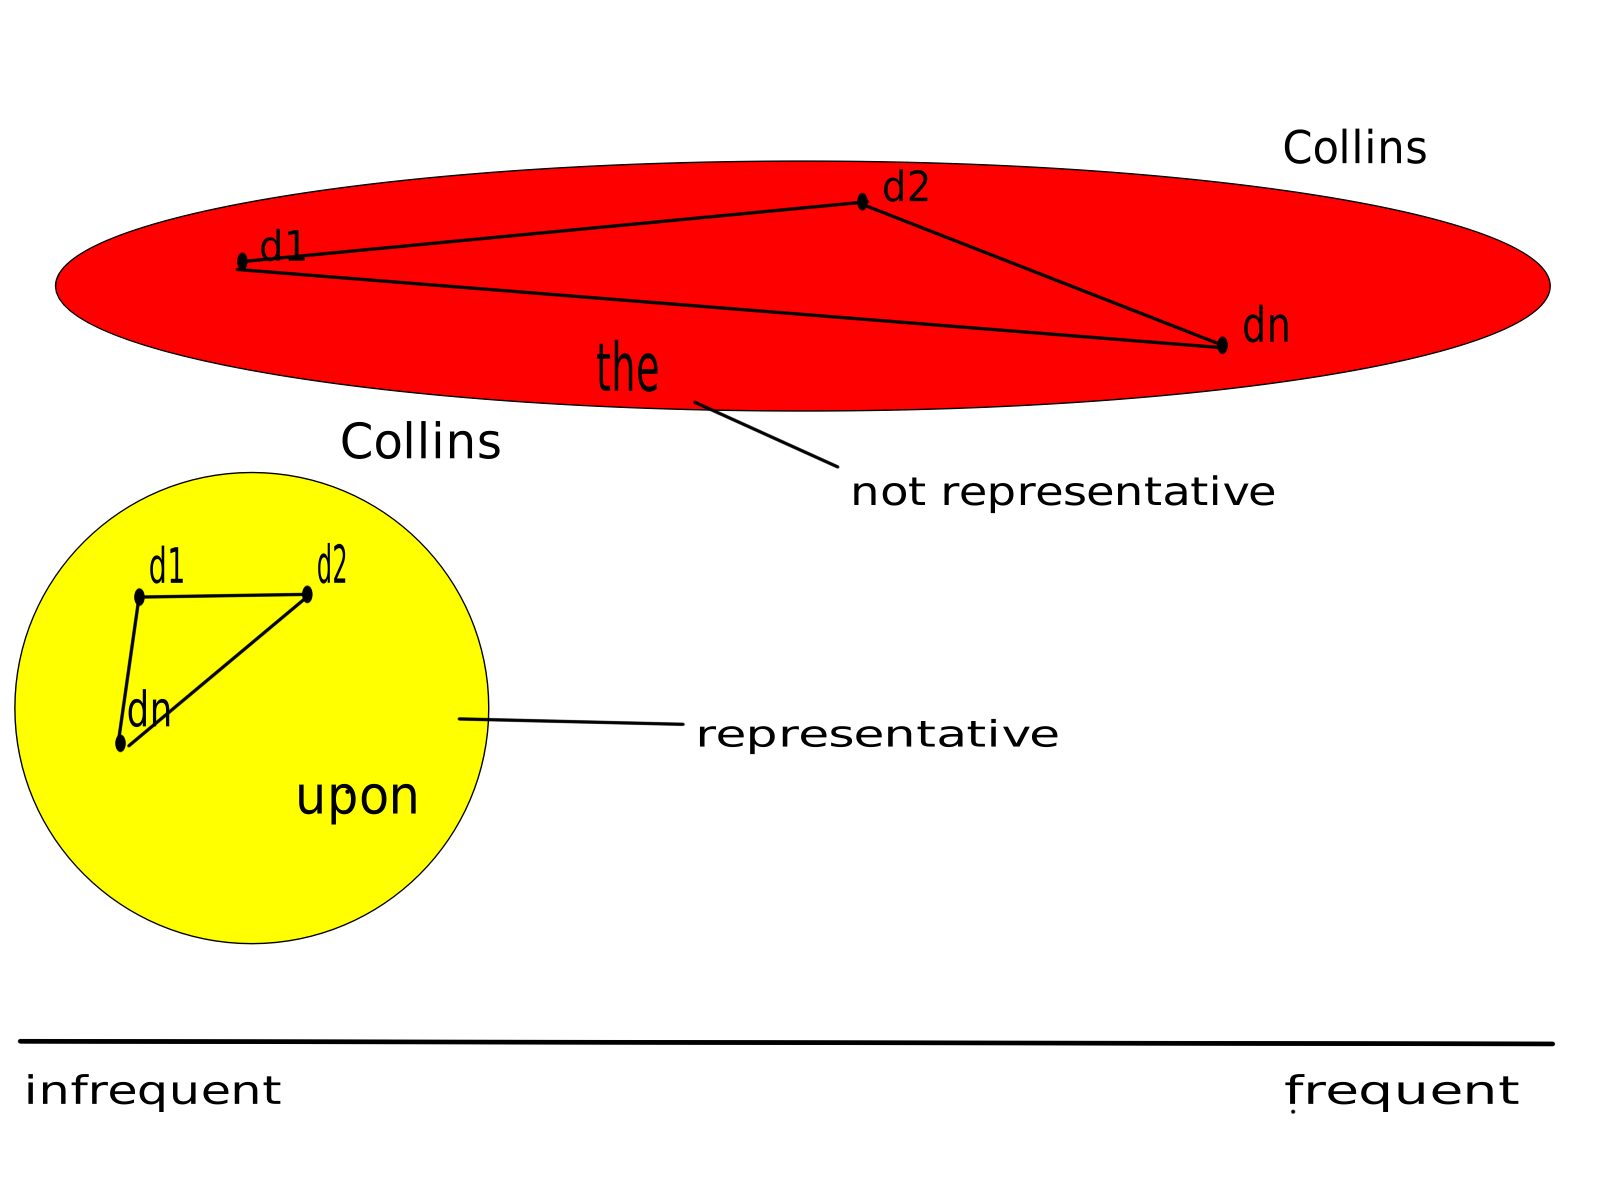
\includegraphics[width=0.4\textwidth]{figures/repres1-fin.png}
  \end{center}
 \end{wrapfigure}
 
However, this analysis is directional in the sense that the degree
of representativeness of a certain feature could be different 
for the opposing set, i.e. there are two different scenarios
for a feature being \emph{different} in the opposing set. 

Case 1. The term $t_i$ is consistent in Collins' set $C$ with a low
frequency, while the same term $t_i$ is consistent in Dickens' set $D$
with a high frequency. 
Thus, the term is representative and distinctive for both sets, 
even though we did not consider the \emph{Representativeness} for set $D$. 
Obviously, the converse could also be true: a consistently high frequency 
for set $C$ and a consistently low frequency for the set $D$.
This first case does not produce any issues for measuring similarity, 
since on the basis of these features there is is reliable similarity 
within sets and accentuated differences between the sets. 


\begin{wrapfigure}{r}{0.4\textwidth}
\caption{\textsc{Distinctiveness}}
{\scriptsize \textsc{Case 1}}\\
  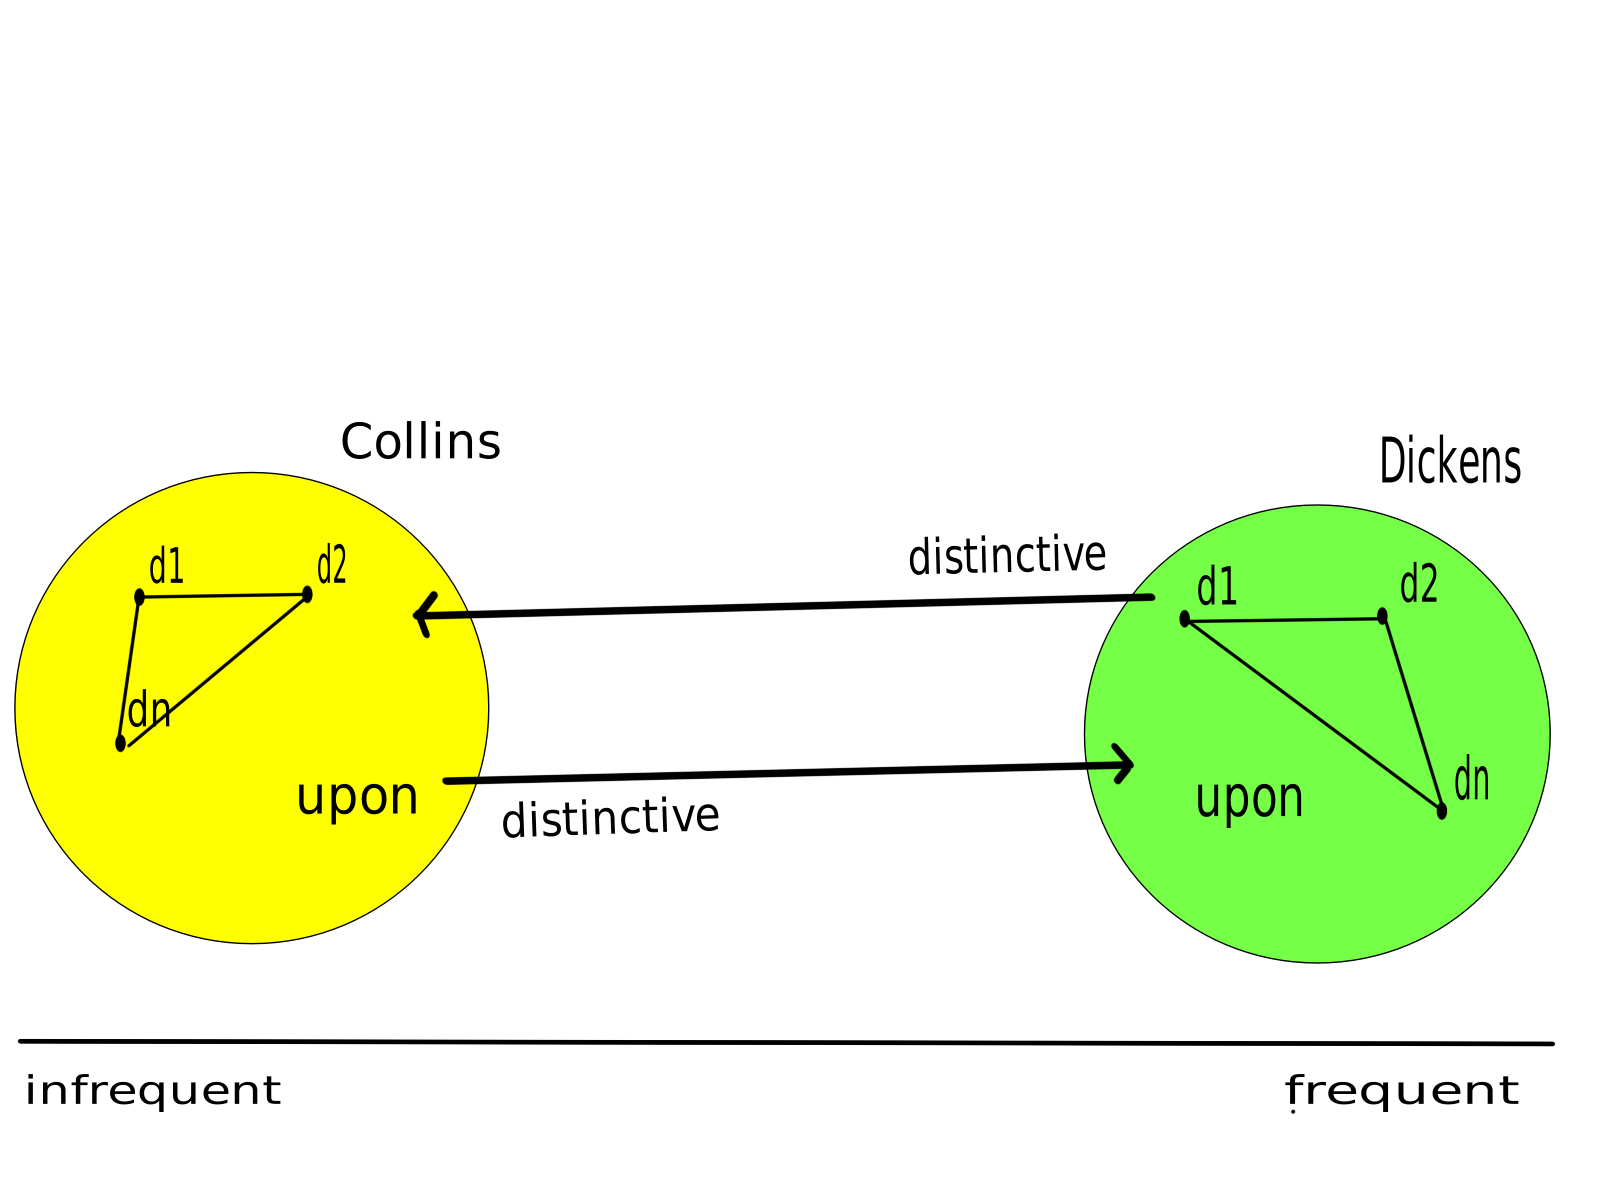
\includegraphics[scale=0.2,width=\linewidth]{figures/distinc1-fin.png}
{\scriptsize \textsc{Case 2}}\\
  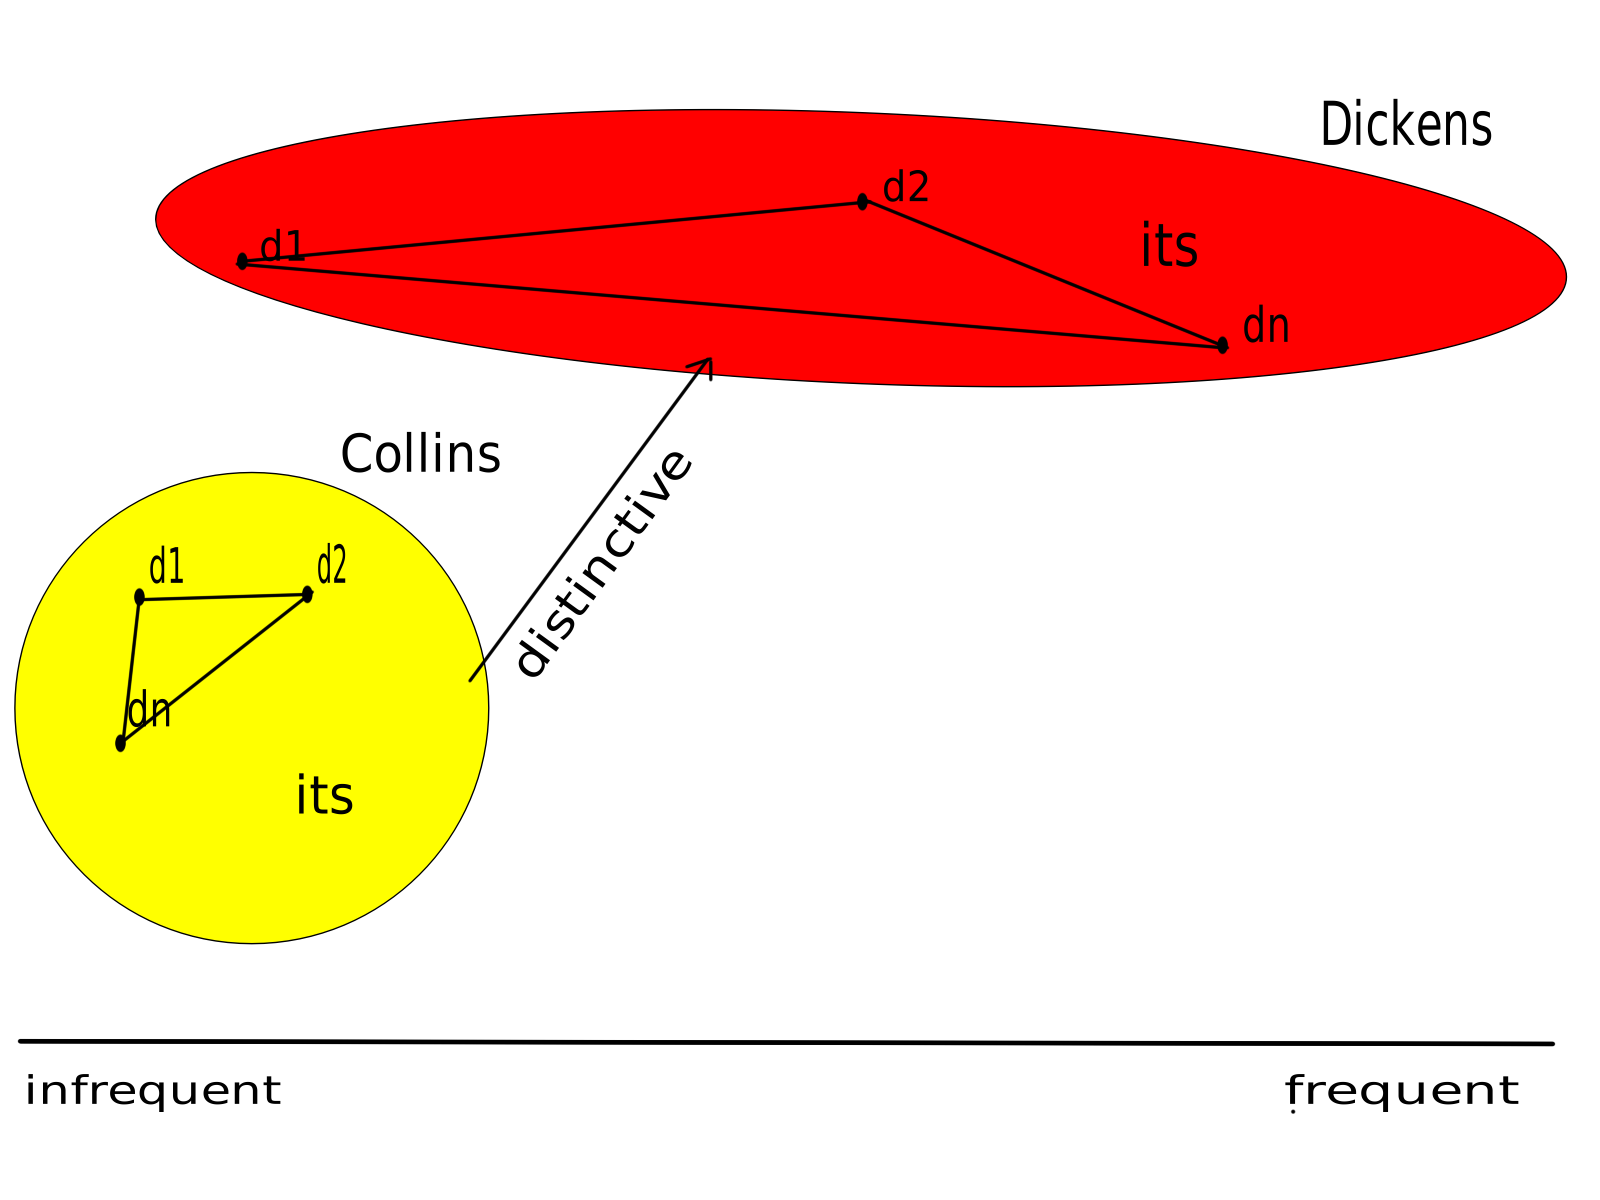
\includegraphics[scale=0.2,width=\linewidth]{figures/distinc2-fin.png}
\end{wrapfigure}


Case 2. The second possibility is the one that may cause issues.
Assuming a representative and distinctive term for set $C$, with a 
frequency either high or low. 
However, the same term is not representative for set $D$ and values 
may fluctuate from high to low. Although this term is not representative 
for $D$, it is distinctive from $C$ to $D$, because it is constant in $C$ 
while not being so in $D$. 
Clustering the data set on the basis of these terms may create noise, 
since it will not show similarities for documents within $D$ and 
may have occasional rather similar values to the ones in $C$ that 
rate it closer to documents in $C$.

In order to identify elements representative and distinctive for both sets,
first, the analysis has to be carried out for both sets and having identified
two separate author profiles, we select those features that are shared
by both.

\subsection{Evaluation of Distinctive Markers} \label{sec:evaluation}
Evaluation in studies of authorship can only be done heuristically
by identifying desirable properties of stylistic markers and
determining means of measuring this property. 
One of these desirable characteristics could be considered 
as stylistic marker's ability to separate the author's set in 
question. 
For instance, having identified a set of discriminatory markers
for Dickens and Collins using a particular method, we evaluate 
that method by testing whether those markers are indeed able to 
cluster the document space appropriately into the two groups of
documents. 
Thus, discrimination ability of a set of distinctive markers
is determined by the overall similarity grouping of documents 
according to those markers. 
Poor discriminators will result in poor clustering, where
authors are not separated well into two groups, while 
good discriminators should be able to divide documents of 
different origin clearly into two different groups. 
This can be quantified by evaluating the clustering result
using the \emph{Adjusted Rand Index} \cite{hubert1985comparing},
which compares the current clustering result to the ideal 
result by pairwise comparison of the groups. 
The returned index is bounded by [-1,1], with 0 being the 
expected value and 1 the highest positive correlation 
between two different clustering versions. 

\section{Experiments}\label{sec:experiments}



\begin{table}
\small 
\caption{Results of Adjusted Rand Index for feature types of word unigrams and POS bigrams.}
 \begin{tabular}{lrrr} \toprule
Test Doc       & word unigrams & POS bigrams & POS trigrams\\ \midrule
D1023     & 0.93  & 0.79  & 0.85 \\
D1400     & 0.93  & 0.66  & 0.93 \\
D19337    & 0.93  & 0.79  & 0.85 \\
D40723    & 0.93  & 0.79  & 0.85 \\
D564      & 0.93  & 0.79  & 0.93 \\
D580      & 0.93  & 0.79  & 0.85 \\
D588      & 0.93  & 0.79  & 0.85 \\
D650      & 0.93  & 0.85  & 0.93 \\
D675      & 0.93  & 0.66  & 0.79 \\
D699      & 0.93  & 0.85  & 0.85 \\
D700      & 0.93  & 0.79  & 0.85 \\
D730      & 0.93  & 0.79  & 0.85 \\
D766      & 0.93  & 0.79  & 0.85 \\
D821      & 0.93  & 0.85  & 0.85 \\
D872      & 0.93  & 0.79  & 0.79 \\
D882      & 0.93  & 0.85  & 0.85 \\
D883      & 0.93  & 0.79  & 0.85 \\
D914      & 0.93  & 0.85  & 0.93 \\
D916      & 0.93  & 0.79  & 0.79 \\
D917      & 0.93  & 0.79  & 0.85 \\
D963      & 0.93  & 0.79  & 0.85 \\
D967      & 0.93  & 0.79  & 0.85 \\
D968      & 0.93  & 0.79  & 0.85 \\
D98       & 0.93  & 0.66  & 0.85 \\
Dal2324   & 0.93  & 0.79  & 0.85 \\
Dal28198  & 0.93  & 0.85  & 0.85 \\
DC1423    & 0.93  & 0.79  & 0.79 \\
C1438     & 0.85  & 0.85  & 0.85 \\
C155      & 0.93  & 0.79  & 0.93 \\
C1586     & 0.93  & 0.79  & 0.85 \\
C1587     & 0.93  & 0.66  & 0.85 \\
C1588     & 0.93  & 0.85  & 0.85 \\
C1621     & 0.93  & 0.93  & 0.85 \\
C1622     & 0.93  & 0.79  & 0.85 \\
C1623     & 0.93  & 0.85  & 0.93 \\
C1624     & 0.85  & 0.85  & 0.85 \\
C1626     & 0.93  & 0.79  & 0.72 \\
C1627     & 0.93  & 0.79  & 0.85 \\
C1628     & 0.93  & 0.79  & 0.85 \\
C1629     & 0.93  & 0.85  & 0.85 \\
C1630     & 0.93  & 0.79  & 0.85 \\
C170      & 0.93  & 0.85  & 0.85 \\
C1895     & 0.93  & 0.85  & 0.85 \\
C1917     & 0.93  & 0.85  & 0.79 \\
C1975     & 0.93  & 0.79  & 0.79 \\
C28367    & 0.93  & 0.85  & 0.93 \\
C3606     & 0.93  & 0.79  & 0.79 \\
C3632     & 0.93  & 0.79  & 0.85 \\
C3633     & 0.93  & 0.79  & 0.79 \\
C4605     & 0.93  & 0.85  & 0.85 \\
C583      & 0.93  & 0.66  & 0.79 \\
C7891     & 0.85  & 0.85  & 0.79 \\
C7893     & 0.93  & 0.79  & 0.79 \\
C7894     & 0.93  & 0.79  & 0.85 \\
\bottomrule
\end{tabular}
\end{table}



\begin{table}
\caption{Dickens' and Collins' highest rated features.}
\begin{tabular}{lllllrr}\toprule[1.2pt]
 \multicolumn{1}{c}{\textbf{No}} & \multicolumn{2}{c}{\textbf{Word unigrams}}&  \multicolumn{2}{c}{\textbf{POS bigrams}} & \multicolumn{2}{c}{\textbf{POS trigrams}}\\
 \cmidrule(r){1-1} 
 \cmidrule(r){2-3} 
\cmidrule(r){4-5} 
 \cmidrule(r){6-7}
    & Dickens	  &  Collins    & Dickens&  Collins& Dickens	  &  Collins   \\\midrule
1   &       upon  &       upon  &  RP.CC  &   NN.TO  &  CC.NN.CC   & IN.VBG.PP. \\
2   &   scarcely  & discovered  &  IN.IN  &   RB.TO  &  NN.CC.RB   &   TO.DT.NN  \\
3   & discovered  &   produced  &  NN.TO  &   RP.CC  &  RB.IN.IN   &  IN.VBG.DT \\
4   &       many  &  interests  & VBG.RP  &  TO.PP.  & CC.VBG.RP   &  PP..JJ.JJ \\
5   &        and  &       left  &  CC.RB  & VBP.VBD  & VBN.RP.CC   &   DT.NN.TO \\
6   &       left  &       many  & CC.VBG  &   NN.NN  &  RB.MD.VB   & VBD.IN.VBG \\
7   &       very  &    useless  &  JJ.CC  &  NNS.NN  & RB.TO.PP.   & VBN.IN.VBG \\
8   &        but  &    attempt  &  NN.CC  &   RB.NN  & CC.VBG.IN   &  DT.NN.PP. \\
9   &       much  &     motive  &  CC.IN  &   NP.NN  & DT.NN.PP.   &   NN.NN.NN \\
10  &     beside  &       only  &  DT.CC  &   RB.JJ  &  RB.JJ.CC   & NN.WDT.PP. \\
11  &     though  &       risk  &  RB.CC  & VBZ.VBD  &  JJ.NN.CC   &  TO.PP..NN \\
12  &       down  & resolution  &  RB.TO  &  CC.WRB  &  IN.IN.DT   &  TO.VB.PP. \\
13  &   produced  &      words  & VBG.JJ  &  CC.VBG  & CC.VBG.CC   & VBD.TO.PP. \\
14  &    several  &  hesitated  &  IN.CC  &  VBG.RP  &  RB.RB.CC   &  RB.TO.PP. \\
15  &       lest  &       very  &  CC.NN  & VBN.PP.  & VBG.RP.CC   & PP..NNS.PP \\
16  &     failed  &   scarcely  & CC.WRB  & NNS.VBP  & NNS.CC.RB   & VBD.NP.NNS \\
17  &    control  &     future  & VBG.CC  &  VBN.TO  &  DT.NN.TO   & PP..NN.POS \\
18  &      great  &     return  & RP.NNS  &   RB.MD  &  CC.JJ.CC   &   PP.DT.NN \\
19  &       such  &      first  & PDT.DT  &  NP.NNS  & RB.CC.VBG   &   DT.NN.PP \\
20  &     indeed  &     failed  &  CC.JJ  &  VB.PP.  &  CC.RB.RB   &  VBD.TO.DT \\
\bottomrule
\end{tabular}
\end{table}




\section{Conclusion}\label{sec:conclusion}







%\nocite{Sag} % items in your bibliography file that are not cited in your text


\bibliographystyle{clin} 
\bibliography{biblio}  

%\appendix



% 
% \section*{Dickens vs. Collins}
% \begin{table}[h!] % Dickens 
% \caption{Dickens' data set as part of the Dickens vs. Collins comparison.}
% \label{table:Dickens-data}
% \scalebox{0.8}{
% \begin{tabular}{c l l l} \\\hline \hline
% \textbf{No.} 	& \textbf{Author} 	& \textbf{Texts} 			& \textbf{Abbr.} \\ \hline
% 1   		& Dickens 		& Bleak House 				& D1023     \\
% 2   		& Dickens		& Great Expectations			& D1400      \\
% 3		& Dickens      		& Little Dorrit     			& D963       \\
% 4		& Dickens      		& David Copperfield     		& D766        \\
% 5		& Dickens      		& A Christmas Carol     		& D19337       \\
% 6   		& Dickens		& Life And Adventures Of Martin Chuzzlewit	& D968        \\
% 7		& Dickens		& The Mystery of Edwin Drood		& D564   \\
% 8		& Dickens      		& A Tale of Two Cities                  & D98      \\
% 9		& Dickens		& Master Humphrey's Clock		& D588           \\
% 10		& Dickens		& The Battle of Life: A Love Story      & D40723              \\
% 11		& Dickens		&Life And Adventures Of Nicholas Nickleby	& D967          \\  
% 12		& Dickens		&Barnaby Rudge      			& D917             \\
% 13		& Dickens		& Sketches of Young Couples		& D916        \\
% 14		& Dickens		& The Uncommercial Traveller            & D914           \\
% 15		& Dickens		& Our Mutual Friend			& D883           \\
% 16		& Dickens		& Pictures From Italy			& D650    \\
% 17		& Dickens		& Sketches by Boz			& D882      \\
% 18		& Dickens		& A Child's History of England       	& D699  \\
% 19		& Dickens		& Reprinted Pieces			& D872   \\
% 20		& Dickens		& Dombey and Son			& D821     \\
% 21		& Dickens		& Oliver Twist				& D730        \\
% 22		& Dickens		&The Old Curiosity Shop			& D700         \\
% 23		& Dickens		& American Notes			& D675         \\
% 24		& Dickens		&The Pickwick Papers			& D580           \\
% 25		& Dickens     (et al.)  & A Budget of Christmas Tales		& Dal28198         \\
% 26		& Dickens (et al.)	& A House to Let			& Dal2324     \\
% 27		& Dickens (/Collins)     & No Thoroughfare			& DC1423       \\ \bottomrule
% \end{tabular}
% }
% \end{table}
% 
% \begin{table}[h!]% Collins 
% \caption{Collins' data set as part of the Dickens vs. Collins comparison.}
% \label{table:Collins-data}
% \scalebox{0.8}{
% \begin{tabular}{c l l l } \\\hline \hline
% \textbf{No.}	& \textbf{Author} 		& \textbf{Texts} 		& \textbf{Abbr.} \\ \hline
% 1		& Collins       		& After Dark			& C1626    \\
% 2		& Collins			& Antonina			& C3606        \\
% 3		& Collins			& Armadale			& C1895  \\
% 4		& Collins			& Man and Wife			& C1586      \\
% 5		& Collins			& Little Novels			& C1630    \\
% 6		& Collins			& Jezebel's Daughter		& C3633    \\
% 7		& Collins			& I Say No			& C1629       \\
% 8		& Collins			& Hide and Seek			& C7893  \\
% 9		& Collins			& Basil				& C4605 \\
% 10		& Collins			& A Rogue's Life		& C1588     \\
% 11		& Collins			& The Woman in White		& C583         \\
% 12		& Collins			& The Two Destinies		& C1624    \\
% 13		& Collins			& The Queen of Hearts		& C1917        \\
% 14		& Collins			& The New Magdalen		& C1623     \\
% 15		& Collins			& The Moonstone			& C155         \\
% 16		& Collins			& The Legacy of Cain		& C1975       \\
% 17		& Collins			& The Law and the Lady		& C1622         \\
% 18		& Collins			& The Haunted Hotel: A Mystery of Modern Venice	&    C170              \\
% 19		& Collins			& The Fallen Leaves		& C7894           \\
% 20		& Collins			& The Evil Genius		& C1627           \\
% 21		& Collins			& No Name			& C1438        \\
% 22		& Collins			& Poor Miss Finch		& C3632           \\
% 23		& Collins			& Rambles Beyond Railways	& C28367         \\
% 24		& Collins			& The Black Robe		& C1587      \\
% 25		& Collins			& Miss or Mrs.?			& C1621          \\
% 26		& Collins			& My Lady's Money		& C1628         \\
% 27		& Collins			& The Dead Alive		& C7891        \\
% \bottomrule
% \end{tabular}
% }
%  \end{table}
% 



\end{document}
